\documentclass[10pt,letterpaper]{article}
\usepackage[utf8]{inputenc}
\usepackage[T1]{fontenc}
\usepackage[margin=0.6in]{geometry}
\usepackage{amsmath,amssymb,mathtools,graphicx,booktabs,xcolor,hyperref}
\setlength{\parindent}{0pt}
\setlength{\parskip}{5pt}
\begin{document}

\section*{Block S2 Exercises: Wheatstone Bridge Analysis via KVL/KCL}

  \textbf{Schedule Window:} Sunday, Oct 18, 4:00--4:55 PM (55 min) ~|~
  \textbf{Total Points:} 34 pts ~|~
  \textbf{Mix:} 1 Calculus/Algebra Derivation, 1 Spec v2 Bridge FR, 1 Graph + Cloze Problem



  \textbf{Core Mastery Goals:} (1) Proving the Wheatstone bridge null-balance ratio $R_1/R_2 = R_3/R_4$ from KCL and KVL; (2) Solving an \emph{unbalanced} bridge where series/parallel formulas fail by writing KCL at the left and right bridge nodes $(V_L, V_R)$ and KVL around meshes containing the central bridge resistor $R_G$; (3) Graphing signed bridge current $I_{LR}(R_4)$ across the balance zero-crossing.


\subsection*{01 $\cdot$ Wheatstone Bridge Null-Balance Condition \& Sensitivity Proof \hfill [Ch. 26 $\cdot$ 10 Points $\cdot$ DERIVE]}

Consider a general DC Wheatstone bridge powered by an ideal source $V_T$ between top node $T$ and grounded bottom node $B$ ($V_B = 0\text{ V}$). Upper-left resistor $R_1$ connects $T \to L$, lower-left resistor $R_2$ connects $L \to B$, upper-right resistor $R_3$ connects $T \to R$, lower-right variable resistor $R_4$ connects $R \to B$, and galvanometer resistance $R_G$ connects $L \to R$ with reference current arrow $I_{LR}$ pointing from $L$ to $R$.

\begin{enumerate}
  \item \textbf{Null-Balance Proof from KCL \& KVL [4 points]:}
    \begin{enumerate}
      \item Suppose the bridge is adjusted so that the galvanometer reads zero current ($I_{LR} = 0$). Using Ohm's law across $R_G$, state the relationship between node potentials $V_L$ and $V_R$, and use KCL at nodes $L$ and $R$ to relate the upper-leg and lower-leg currents ($I_1$ vs. $I_2$, and $I_3$ vs. $I_4$).
      \item Write KVL around the upper loop ($T \to L \to R \to T$) and lower loop ($L \to B \to R \to L$), or apply voltage division on each leg, to prove that $I_{LR} = 0$ if and only if:
      $$\frac{R_1}{R_2} = \frac{R_3}{R_4} \quad \Longleftrightarrow \quad R_1 R_4 = R_2 R_3.$$
      \item Explain briefly why changing the source voltage $V_T$ or the galvanometer resistance $R_G$ does \emph{not} shift the balance resistance $R_{4,\text{bal}}$.
    \end{enumerate}
  
  \item \textbf{Exact Unbalanced Bridge Current \& Calculus Sensitivity Derivative [6 points]:}
    \begin{enumerate}
      \item Fix $V_T = 15.0\text{ V}$, $R_1 = 150\ \Omega$, $R_2 = 300\ \Omega$, $R_3 = 150\ \Omega$, and $R_G = 100\ \Omega$, leaving $R_4 \ge 0$ as a continuous variable. Write KCL at nodes $L$ and $R$ and eliminate $V_L, V_R$ (or find the Th\'evenin equivalent of each bridge leg) to prove that the signed bridge current from $L$ to $R$ is:
      $$I_{LR}(R_4) = \frac{300 - R_4}{6000 + 70 R_4}\text{ A} = \frac{300 - R_4}{6.00 + 0.0700 R_4}\text{ mA}.$$ \textbf{[4 pts]}
      \item Differentiate $I_{LR}(R_4)$ with respect to $R_4$ to evaluate the bridge sensitivity $\left.\dfrac{dI_{LR}}{dR_4}\right|_{R_4 = R_{4,\text{bal}}}$ (in $\mu\text{A}/\Omega$) at the null-balance point. \textbf{[2 pts]}
    \end{enumerate}
  
\end{enumerate}
\vspace{1.2in}


\newpage



\subsection*{02 $\cdot$ Unbalanced Wheatstone Bridge Nodal \& Mesh Analysis \hfill [Ch. 26 $\cdot$ 14 Points $\cdot$ FR + SPEC V2]}

In the Spec v2 Wheatstone bridge below, an ideal DC source $V_T = 15.0\text{ V}$ supplies top node $T$ relative to grounded bottom node $B$ ($V_B = 0\text{ V}$). The four bridge arms are $R_1 = 150\ \Omega$ ($T \to L$), $R_2 = 300\ \Omega$ ($L \to B$), $R_3 = 150\ \Omega$ ($T \to R$), and $R_4 = 150\ \Omega$ ($R \to B$), with central bridge resistor $R_G = 100\ \Omega$ connected between nodes $L$ and $R$.

\begin{center}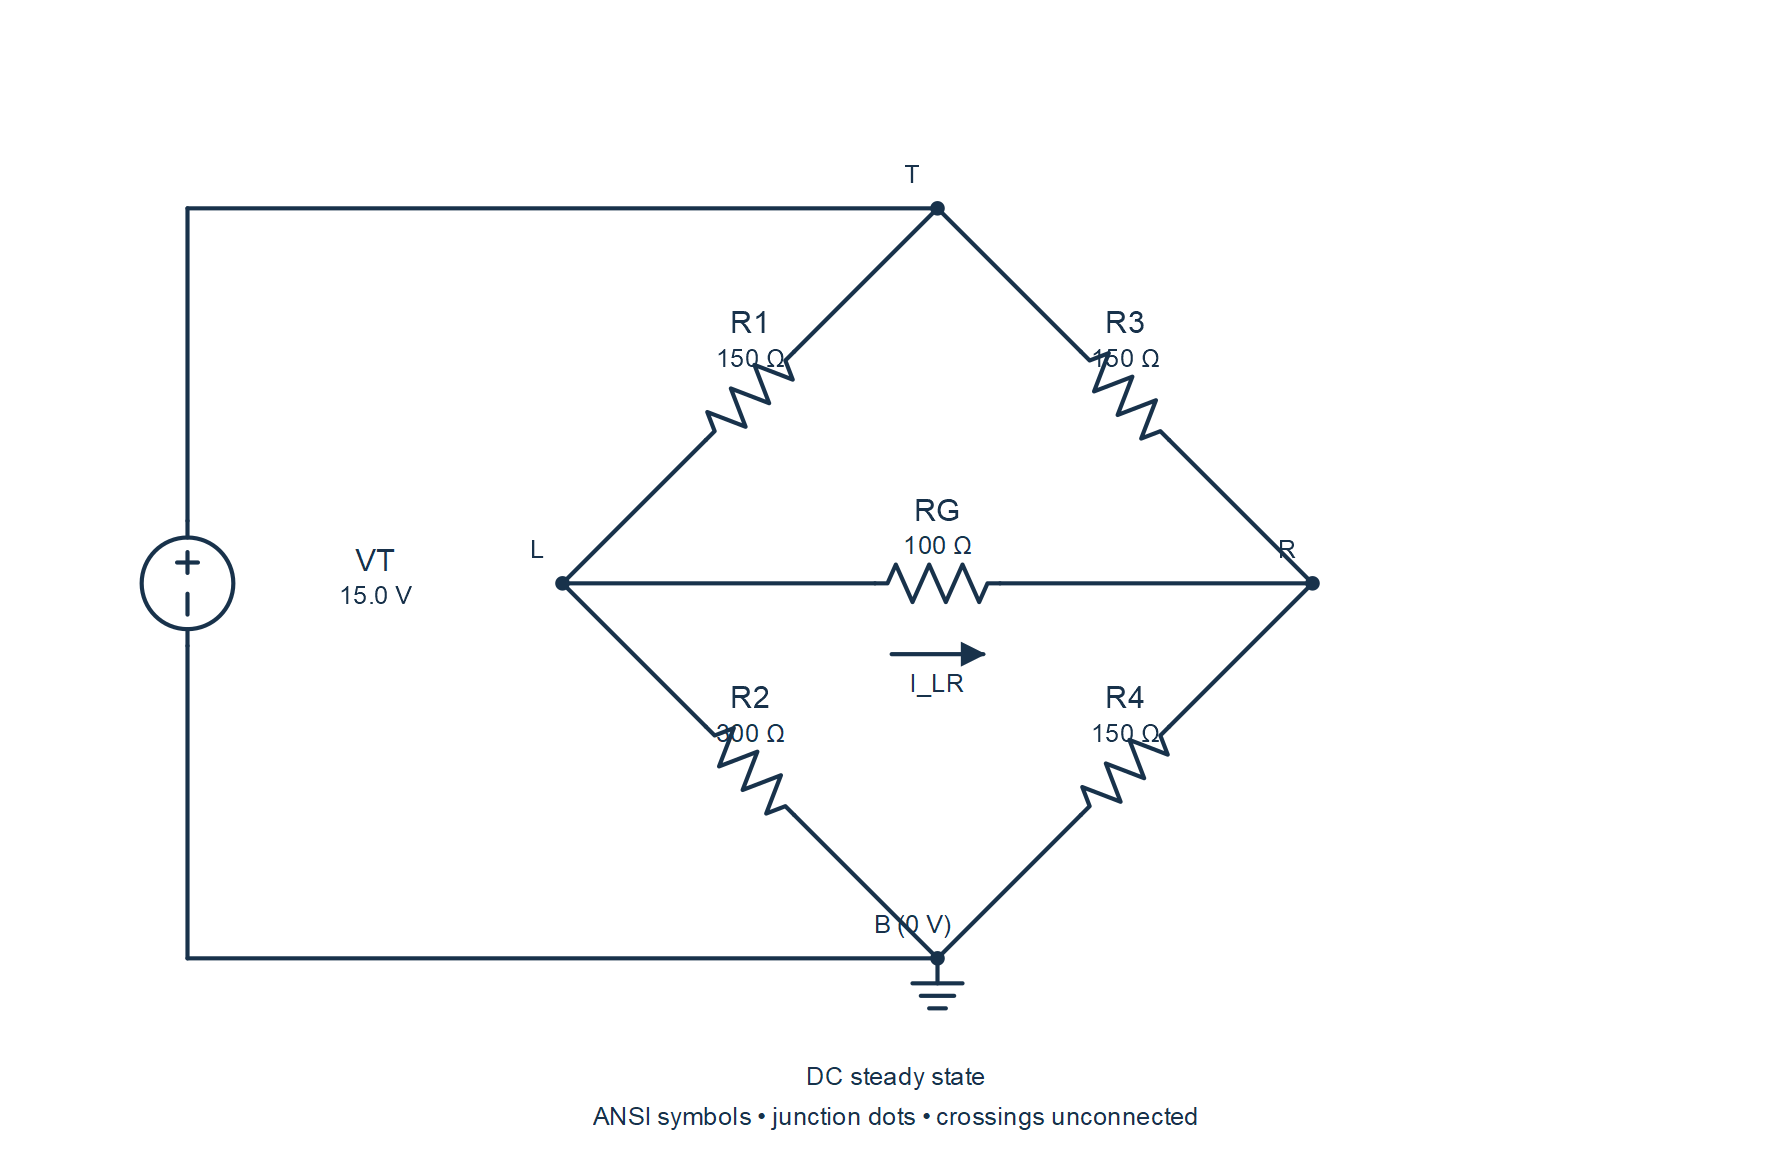
\includegraphics[width=0.82\linewidth]{day1_assets/s2-q2-unbalanced-bridge.png}\end{center}

\begin{enumerate}
  \item \textbf{Why Elementary Series/Parallel Reduction Fails [2 points]:} Explain in one or two sentences why neither $(R_1, R_2)$ nor $(R_1, R_3)$ are in simple series or simple parallel when $R_G = 100\ \Omega$ is present.
  \item \textbf{KCL Nodal System \& KVL Bridge Mesh [4 points]:}
    \begin{enumerate}
      \item Write the KCL equation at node $L$ in terms of the unknown node potentials $V_L$ and $V_R$, and clear fractions to obtain a linear equation of the form $a V_L + b V_R = c$.
      \item Write the KCL equation at node $R$ in terms of $V_L$ and $V_R$, and clear fractions to obtain a second linear equation.
      \item Write the KVL loop equation around the upper triangular mesh ($T \to L \to R \to T$) in terms of branch currents $I_1, I_{LR}, I_3$.
    \end{enumerate}
  
  \item \textbf{Solving for Node Voltages \& Signed Bridge Current [5 points]:} Solve your $2\times 2$ linear system for the exact fractions and three-significant-figure decimal values of $V_L$ and $V_R$ (in $\text{V}$). Calculate the signed bridge current $I_{LR} = \frac{V_L - V_R}{R_G}$ (in $\text{mA}$) and state whether current flows from $L \to R$ or from $R \to L$.
  \item \textbf{All Leg Currents \& Total Equivalent Resistance $R_{\text{eq}}$ [3 points]:} Compute the four leg currents $I_1, I_2, I_3, I_4$ (in $\text{mA}$), find the total source current $I_{\text{src}} = I_1 + I_3 = I_2 + I_4$ leaving node $T$, and determine the total equivalent resistance $R_{\text{eq}} = \frac{V_T}{I_{\text{src}}}$ of the entire 5-resistor bridge network across the $15.0\text{ V}$ source.
\end{enumerate}
\vspace{1.2in}


\newpage



\subsection*{03 $\cdot$ Bridge Current Curve $I_{LR}(R_4)$ \& Conceptual Cloze \hfill [Ch. 26 $\cdot$ 10 Points $\cdot$ DRAW + CLOZE]}

\subsubsection*{Part A: Draw the Effect --- Signed Bridge Current vs. Lower-Right Resistance [6 points --- DRAW]}
Consider the bridge from Exercise 02 ($V_T = 15.0\text{ V}, R_1 = 150\ \Omega, R_2 = 300\ \Omega, R_3 = 150\ \Omega, R_G = 100\ \Omega$) as the lower-right resistor $R_4$ is varied continuously from $0\ \Omega$ to $600\ \Omega$.
\begin{enumerate}
  \item Evaluate $I_{LR}(R_4)$ (in $\text{mA}$) at four landmark resistances: (1) short-circuit $R_4 = 0\ \Omega$, (2) the Exercise 02 operating point $R_4 = 150\ \Omega$, (3) the null-balance resistance $R_{4,\text{bal}}$, and (4) the open-circuit limit $R_4 \to \infty$. \textbf{[2 pts]}
  \item On the coordinate grid below, plot the signed bridge current $I_{LR}$ (\textbf{dependent variable}, vertical axis, in $\text{mA}$) vs. lower-right resistance $R_4$ (\textbf{independent variable}, horizontal axis, in $\Omega$) for $0 \le R_4 \le 600\ \Omega$. Explicitly mark and label the $y$-intercept at $R_4 = 0$, the Exercise 02 operating point at $R_4 = 150\ \Omega$, the zero-crossing balance point at $R_{4,\text{bal}}$, and the dashed horizontal asymptote as $R_4 \to \infty$. \textbf{[4 pts]}
\end{enumerate}

\begin{center}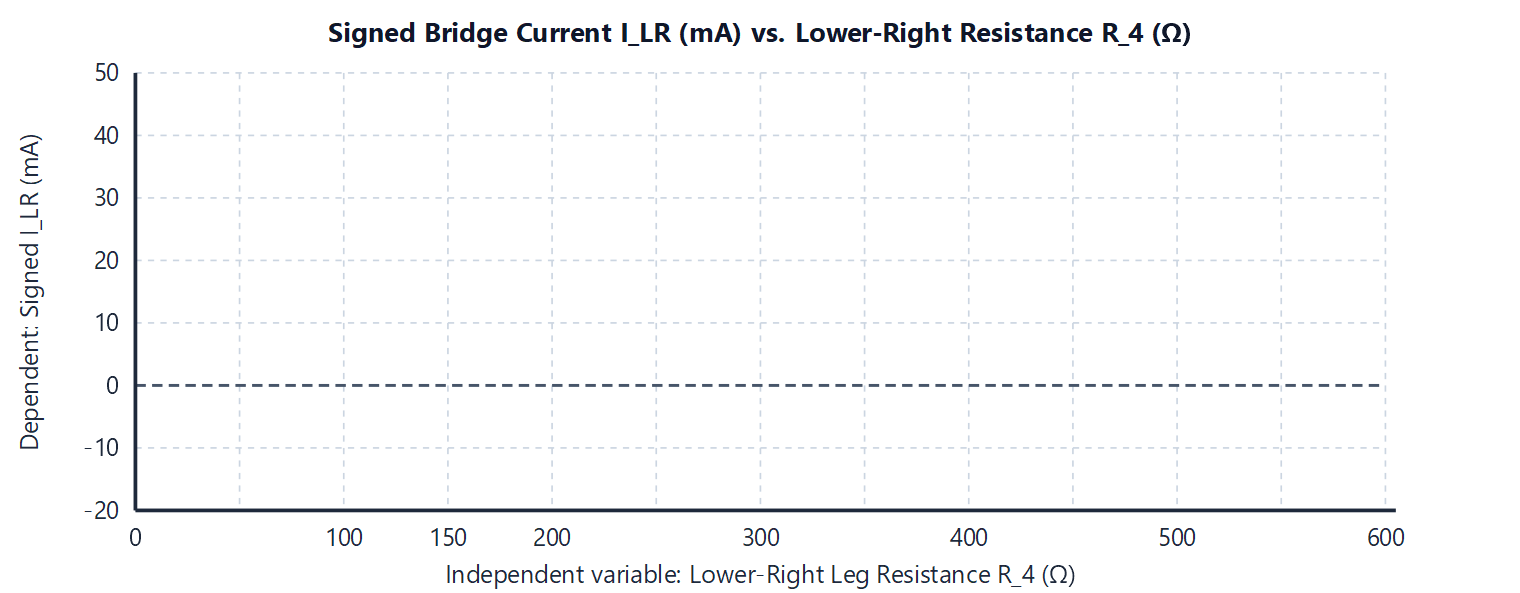
\includegraphics[width=0.82\linewidth]{day1_assets/s2-q3-grid-blank.png}\end{center}

\subsubsection*{Part B: Wheatstone Bridge Conceptual Cloze [4 points --- 0.5 point each]}

  \textbf{WORD BANK:} ~
  \texttt{equal to} $\cdot$
  \texttt{zero} $\cdot$
  \texttt{$300\ \Omega$} $\cdot$
  \texttt{$75.0\ \Omega$} $\cdot$
  \texttt{from $L$ to $R$} $\cdot$
  \texttt{from $R$ to $L$} $\cdot$
  \texttt{unchanged} $\cdot$
  \texttt{doubled} $\cdot$
  \texttt{both an open and a short circuit} $\cdot$
  \texttt{Kirchhoff's junction rule}


\begin{enumerate}
  \item A Wheatstone bridge is balanced when the central galvanometer current $I_G$ is \underline{\hspace{1.8in}}, which requires the node potentials to satisfy $V_L$ \underline{\hspace{1.8in}} $V_R$.
  \item For $R_1 = 150\ \Omega$, $R_2 = 300\ \Omega$, and $R_3 = 150\ \Omega$, the unique lower-right resistance that balances the bridge is $R_{4,\text{bal}} =$ \underline{\hspace{1.8in}}.
  \item When $R_4 < R_{4,\text{bal}}$ (for example, $R_4 = 150\ \Omega$), node $R$ is pulled closer to ground than node $L$ ($V_R < V_L$), so current in $R_G$ flows \underline{\hspace{1.8in}}.
  \item When $R_4 > R_{4,\text{bal}}$ (for example, $R_4 = 500\ \Omega$), $V_R > V_L$ and current in $R_G$ reverses to flow \underline{\hspace{1.8in}}.
  \item If the DC source voltage $V_T$ is doubled from $15.0\text{ V}$ to $30.0\text{ V}$ while the bridge is balanced, the balance resistance $R_{4,\text{bal}}$ remains \underline{\hspace{1.8in}}.
  \item At exact null balance ($I_{LR} = 0$ and $V_L = V_R$), the equivalent resistance $R_{\text{eq}}$ across the source can be found by treating $R_G$ as \underline{\hspace{1.8in}}.
  \item Setting up the nodal equations $\frac{V_L - V_T}{R_1} + \frac{V_L}{R_2} + \frac{V_L - V_R}{R_G} = 0$ is a direct application of \underline{\hspace{1.8in}}.
\end{enumerate}

\end{document}
